\documentclass[11pt,a4paper]{article}

\usepackage[utf8]{inputenc}
\usepackage[T1]{fontenc}
\IfFileExists{danish.ldf}{\usepackage[danish]{babel}}{}
\IfFileExists{lmodern.sty}{\usepackage{lmodern}}{}
\usepackage[margin=2.6cm]{geometry}
\usepackage{amsmath,amssymb}
\usepackage{booktabs}
\usepackage{threeparttable}
\usepackage{graphicx}
\usepackage{caption}
\usepackage[authoryear,round]{natbib}
\usepackage{setspace}
\usepackage[hidelinks]{hyperref}

\captionsetup{font=small,labelfont=bf}
\setstretch{1.2}
\setlength{\parskip}{0.45em}
\setlength{\parindent}{0pt}
\graphicspath{{generated/}}

% Alle tal kommer fra analysen (python3 run.py) og simulationerne (tests/monte_carlo.py)
% Genereret af src/latex.py. Rediger ikke manuelt.
\newcommand{\SampleStart}{august 2010}
\newcommand{\SampleEnd}{oktober 2026}
\newcommand{\NObs}{195}
\newcommand{\DataTil}{16.\,10.\,2026}
\newcommand{\PartialNote}{Den sidste måned er ufuldstændig og løber til 16.\ oktober.}
\newcommand{\BetaEMLC}{\ensuremath{-1{,}70}}
\newcommand{\TEMLC}{\ensuremath{-19{,}41}}
\newcommand{\RtoEMLC}{\ensuremath{0{,}74}}
\newcommand{\BetaCEW}{\ensuremath{-1{,}25}}
\newcommand{\BetaLok}{\ensuremath{-0{,}45}}
\newcommand{\BetaEMB}{\ensuremath{-1{,}05}}
\newcommand{\BetaEMLCctrl}{\ensuremath{-1{,}63}}
\newcommand{\OilEMLC}{\ensuremath{0{,}020}}
\newcommand{\TOilEMLC}{\ensuremath{1{,}04}}
\newcommand{\DiffBeta}{\ensuremath{-0{,}65}}
\newcommand{\DiffT}{\ensuremath{-5{,}90}}
\newcommand{\ValutaAndel}{\ensuremath{74}}
\newcommand{\AsymOp}{\ensuremath{-1{,}90}}
\newcommand{\AsymNed}{\ensuremath{-1{,}43}}
\newcommand{\AsymP}{\ensuremath{0{,}09}}
\newcommand{\OosRto}{\ensuremath{-1{,}51}}
\newcommand{\OosP}{\ensuremath{0{,}91}}
\newcommand{\RollMin}{\ensuremath{-2{,}25}}
\newcommand{\RollMax}{\ensuremath{-1{,}29}}
\newcommand{\RollLast}{\ensuremath{-1{,}30}}
\newcommand{\SepMonth}{september 2026}
\newcommand{\SepUSD}{\ensuremath{2{,}01}}
\newcommand{\SepEMLC}{\ensuremath{-2{,}58}}
\newcommand{\DomI}{understøttes}
\newcommand{\DomII}{understøttes}
\newcommand{\DomIII}{understøttes}
\newcommand{\DomIV}{understøttes ikke}
\newcommand{\DomV}{understøttes ikke}
\newcommand{\DomVI}{understøttes ikke}
\newcommand{\RateLok}{\ensuremath{-2{,}51}}
\newcommand{\TRateLok}{\ensuremath{-6{,}03}}
\newcommand{\RateEMB}{\ensuremath{-5{,}33}}
\newcommand{\TRateEMB}{\ensuremath{-9{,}87}}
\newcommand{\AsymOpCEW}{\ensuremath{-1{,}40}}
\newcommand{\AsymNedCEW}{\ensuremath{-1{,}05}}
\newcommand{\AsymPCEW}{\ensuremath{0{,}03}}
\newcommand{\SepEMLCmodel}{\ensuremath{-3{,}56}}
\newcommand{\SepEMB}{\ensuremath{-3{,}80}}
\newcommand{\SepEMBmodel}{\ensuremath{-2{,}47}}
\newcommand{\SepTekst}{EM-lokalvaluta klarede sig altså bedre end den historiske sammenhæng tilsiger, mens hård valuta klarede sig dårligere. Det er konsistent med, at Fed-forhøjelsen især ramte gennem de amerikanske renter, som hård valuta er mest følsom over for.}
\newcommand{\KonklKanal}{og med begge valutaproxyer kommer hovedparten gennem valutaen}
\newcommand{\KonklSignal}{Jeg finder ingen evidens for, at dollaren kan bruges som signal med en måneds forsinkelse; eksponeringen viser sig samtidig.}
\newcommand{\KonklAsym}{Den forhåndsfastlagte test finder ikke signifikant asymmetri, men testen har begrænset styrke.}
\newcommand{\AfeEMLC}{\ensuremath{-1{,}27}}
\newcommand{\TAfeEMLC}{\ensuremath{-13{,}18}}
\newcommand{\AfeCEW}{\ensuremath{-0{,}95}}
\newcommand{\AfeRtoCEW}{\ensuremath{0{,}61}}
\newcommand{\BredRtoCEW}{\ensuremath{0{,}80}}
\newcommand{\AfeLok}{\ensuremath{-0{,}32}}
\newcommand{\TAfeLok}{\ensuremath{-7{,}13}}
\newcommand{\SpotBeta}{\ensuremath{-1{,}13}}
\newcommand{\SpotAndel}{\ensuremath{67}}
\newcommand{\SpotRest}{\ensuremath{-0{,}56}}
\newcommand{\TSpotRest}{\ensuremath{-11{,}82}}
\newcommand{\CewAndel}{\ensuremath{74}}
\newcommand{\AndelMin}{\ensuremath{67}}
\newcommand{\AndelMax}{\ensuremath{74}}
\newcommand{\AfeRtoEMLC}{\ensuremath{0{,}55}}
\newcommand{\AfeLokSpot}{\ensuremath{-0{,}44}}
\newcommand{\AfeEMB}{\ensuremath{-0{,}77}}
\newcommand{\VixPEMLC}{\ensuremath{0{,}12}}
\newcommand{\NoVixPCEW}{\ensuremath{0{,}03}}
\newcommand{\SpotOp}{\ensuremath{-1{,}29}}
\newcommand{\SpotNed}{\ensuremath{-0{,}93}}
\newcommand{\VixPCEW}{\ensuremath{0{,}05}}
\newcommand{\VixDiffCEW}{\ensuremath{-0{,}30}}
\newcommand{\VixPSpot}{\ensuremath{0{,}02}}
\newcommand{\NoVixPSpot}{\ensuremath{0{,}01}}

\IfFileExists{generated/mc.tex}{% Genereret af tests/monte_carlo.py. Rediger ikke manuelt.
\newcommand{\MCR}{2.000}
\newcommand{\MCCWsize}{\ensuremath{3{,}2}}
\newcommand{\MCCWsizeSE}{\ensuremath{0{,}4}}
\newcommand{\MCCWsizeAll}{\ensuremath{3{,}0}}
\newcommand{\MCCWsizeAllSE}{\ensuremath{0{,}4}}
\newcommand{\MCPowCEW}{\ensuremath{63{,}6}}
\newcommand{\MCPowCEWSE}{\ensuremath{1{,}1}}
\newcommand{\MCPowEMLC}{\ensuremath{46{,}9}}
\newcommand{\MCPowEMLCSE}{\ensuremath{1{,}1}}
\newcommand{\MCSizeAsym}{\ensuremath{5{,}5}}
\newcommand{\MCSizeAsymSE}{\ensuremath{0{,}5}}
\newcommand{\MCBetaOp}{\ensuremath{-0{,}999}}
\newcommand{\MCBetaNed}{\ensuremath{-0{,}598}}
\newcommand{\MCBetaEMB}{\ensuremath{-0{,}398}}
}{}

\hyphenation{penge-markeds-instru-menter valuta-proxy valuta-proxyer lokal-valuta-obligationer}

\begin{document}
\renewcommand{\tablename}{Tabel}
\renewcommand{\figurename}{Figur}
\renewcommand{\refname}{Litteraturliste}
\renewcommand{\contentsname}{Indholdsfortegnelse}

% ------------------------------------------------------------------ Forside
\begin{titlepage}
\centering
\vspace*{1.5cm}
{\Large\bfseries KØBENHAVNS UNIVERSITET\par}
\vspace{0.2cm}
{\large DET SAMFUNDSFAGLIGE FAKULTET\par}
{\large Økonomisk Institut\par}
\vspace{3cm}
{\LARGE\bfseries Hvor følsomme er emerging markets-obligationer i lokalvaluta over for den amerikanske dollar, og gennem hvilken kanal virker effekten?\par}
\vspace{2.5cm}
{\large Albert Claes Poulsen\par}
\vspace{0.2cm}
{\normalsize BSc Økonomi, 2.\ år, Københavns Universitet\par}
{\normalsize \href{mailto:gbl255@alumni.ku.dk}{gbl255@alumni.ku.dk}\par}
\vspace{1.2cm}
{\normalsize Selvstændigt analyseprojekt\par}
{\normalsize 23.\ oktober 2026\par}
\vfill
{\small Data til og med \DataTil. Kode og data: \url{https://github.com/ACP-dev1/dollar-em}\par}
\end{titlepage}

\tableofcontents
\newpage

% ------------------------------------------------------------------ Introduktion
\section*{Introduktion}
\addcontentsline{toc}{section}{Introduktion}

Mange investeringscases for emerging markets (EM) bygger på en forventning om en svagere amerikansk dollar. Argumentet er, at en svag dollar letter finansieringen for EM-lande, sænker værdien af deres dollargæld og trækker kapital mod de højere renter i EM. Dollaren svækkedes gennem sommeren 2026, men vendte kraftigt i september efter Federal Reserves første renteforhøjelse siden 2023. Det gør det relevant at undersøge, hvor meget en dollarvending egentlig betyder for en portefølje af EM-obligationer, og gennem hvilken kanal effekten virker.

På denne baggrund undersøges følgende: \emph{Hvor følsomme er emerging markets-obligationer i lokalvaluta over for den amerikanske dollar, og gennem hvilken kanal virker effekten?}

For at belyse spørgsmålet anvendes månedlige data fra \SampleStart{} til \SampleEnd{} for tre investerbare børshandlede fonde: EM-statsobligationer i lokalvaluta, en kurv af EM-valutaer og EM-statsobligationer i dollar. Dollarfølsomheden estimeres med OLS, og afkastet på lokalvalutaobligationerne opdeles i en valutadel og en restpost. Seks hypoteser og deres forventede fortegn blev skrevet ned, før analysen blev kørt på de rigtige data. Robusthedstjek, som ikke var fastlagt på forhånd, er markeret som eksplorative.

Analysen viser, at en stigning på 1\,\% i Feds brede dollarindeks er forbundet med et afkast på \BetaEMLC\,\% på EM-obligationer i lokalvaluta. Med et dollarindeks, der ikke selv indeholder EM-valutaer, er betaen \AfeEMLC, hvilket viser, at en del af den oprindelige sammenhæng er mekanisk, men at hovedresultatet holder. Valutaen står for mellem \AndelMin{} og \AndelMax\,\% af dollarfølsomheden afhængigt af, hvordan valutadelen måles. Restposten er negativ i alle specifikationer, men den kan ikke entydigt tolkes som en rentekanal. Desuden smitter de amerikanske renter tydeligt af på EM-obligationerne, særligt i hård valuta. Der findes derimod ingen evidens for, at dollarens udvikling i én måned kan forudsige næste måneds afkast.

Samlet set viser analysen, at en position i EM-obligationer i lokalvaluta i praksis også er en position på en svagere dollar. Det er en vigtig pointe for en investor, fordi diversifikationen mod dollaren dermed er mindre, end porteføljens navn antyder.

% ------------------------------------------------------------------ 1 Teori
\section{Teoretisk ramme}

Følgende afsnit opstiller en simpel ramme for, hvordan dollaren kan påvirke afkastet på en obligation i lokalvaluta målt i dollar.

For en investor, der måler sit afkast i dollar, kan afkastet på en EM-obligation i lokalvaluta tilnærmelsesvis skrives som
\begin{equation}\label{eq:teori}
r^{EMLC}_t \;\approx\; \underbrace{y_{t-1}}_{\text{carry}} \;-\; \underbrace{D \, \Delta y_t}_{\text{kursdel}} \;+\; \underbrace{\Delta e_t}_{\text{valutadel}},
\end{equation}
hvor $y$ er den lokale rente, $D$ er obligationens varighed, og $\Delta e_t$ er ændringen i værdien af den lokale valuta målt i dollar. Ligningen viser, at dollaren kan påvirke afkastet gennem to kanaler.

Den første er \emph{valutakanalen}. Når dollaren styrkes, falder værdien af EM-valutaerne målt i dollar, så $\Delta e_t < 0$. Denne effekt er mekanisk og rammer alle aktiver i lokalvaluta, uanset hvad der sker med renten.

Den anden er \emph{rentekanalen}. \citet{hofmann2020} viser, at en stærkere dollar strammer de finansielle forhold i EM og hæver risikopræmien på obligationer i lokalvaluta. Det svarer til, at $\Delta y_t > 0$, så kursdelen bliver negativ. Mekanismen hænger sammen med, at mange EM-låntagere og deres udenlandske investorer har gæld i dollar, så en stærkere dollar svækker deres balancer og risikovillighed \citep{avdjiev2019}. \citet{verdelhan2018} viser desuden, at en fælles dollarfaktor forklarer en stor del af variationen i bilaterale valutakurser, hvilket understøtter, at dollaren er en systematisk risikofaktor.

Rammen giver tre forudsigelser. For det første bør obligationer i lokalvaluta have en negativ dollarbeta. For det andet bør de være mere dollarfølsomme end EM-obligationer i dollar (hård valuta), som ikke har en valutadel. For det tredje bør en del af følsomheden, men ikke nødvendigvis hele, komme fra valutaen.

% ------------------------------------------------------------------ 2 Data og metode
\section{Data og metode}

\subsection{Data}

Analysen bygger på månedlige data fra \SampleStart{} til \SampleEnd{} ($N=\NObs$). \PartialNote{} Alle serier måles ved månedens sidste handelsdag, og fondskurserne er justeret for udlodninger, så afkastene er totalafkast inklusive carry. Afkast måles som log-afkast i procent i dollar.

\begin{itemize}\setlength\itemsep{0.1em}
  \item \textbf{EMLC}: VanEck J.P.\ Morgan EM Local Currency Bond ETF. Statsobligationer udstedt i lokalvaluta.
  \item \textbf{CEW}: WisdomTree Emerging Currency Strategy ETF. En ligevægtet kurv af EM-valutaer, investeret i korte pengemarkedsinstrumenter, så afkastet indeholder både spotkurs og kort carry.
  \item \textbf{Spotkurv}: ligevægtet spotafkast på de syv valutaer i J.P.\ Morgan GBI-EM, som Federal Reserve offentliggør dagligt (BRL, MXN, ZAR, INR, CNY, MYR og THB). Ingen carry.
  \item \textbf{EMB}: iShares J.P.\ Morgan USD EM Bond ETF. EM-statsobligationer i dollar, uden direkte valutarisiko.
  \item \textbf{Dollar}: Feds brede, handelsvægtede dollarindeks, som også indeholder EM-valutaer, samt indekset mod avancerede økonomier, som ikke gør.
  \item \textbf{Kontroller}: Brent-olie, den amerikanske 10-årige statsrente og VIX.
\end{itemize}

Data er hentet fra FRED (Federal Reserve Bank of St.\ Louis) og Yahoo Finance. En fordel ved at bruge børshandlede fonde er, at afkastene er investerbare og frit tilgængelige. En ulempe er, at fondene har gebyrer og ikke følger de underliggende indeks perfekt. Det ideelle datagrundlag ville være J.P.\ Morgan GBI-EM-indekset i både en valutasikret og en ikke-valutasikret version, men det kræver adgang til Bloomberg eller lignende.

\subsection{Metode}

Dollarfølsomheden estimeres med regressionen
\begin{equation}\label{eq:main}
r_{i,t} = \alpha_i + \beta_i\, \Delta \mathrm{USD}_t + \gamma_i' Z_t + \varepsilon_{i,t},
\end{equation}
hvor $\Delta \mathrm{USD}_t$ er log-ændringen i dollarindekset, og $Z_t$ indeholder ændringen i olieprisen og i den amerikanske 10-årige rente. Regressionen er samtidig, så $\beta_i$ måler eksponeringen mod dollaren og ikke en kausal effekt. Standardfejlene er beregnet efter \citet{newey1987} med tre lags, så de er robuste over for heteroskedasticitet og autokorrelation.

For at opdele dollarfølsomheden tilnærmes valutadelen i ligning~\eqref{eq:teori} med en proxy $r^{FX}$, enten CEW eller spotkurven, og der defineres en restpost
\begin{equation}
r^{rest}_t \equiv r^{EMLC}_t - r^{FX}_t .
\end{equation}
Da restposten er defineret som en forskel, summerer betaerne per konstruktion: $\beta^{EMLC}=\beta^{FX}+\beta^{rest}$. Det er en regneidentitet og ikke en validering af opdelingen. Restposten indeholder kursdelen fra ligning~\eqref{eq:teori}, men også forskellen mellem EMLC's landevægte og proxyens vægte og, for CEW, forskellen i carry. Den kan derfor ikke uden videre tolkes som en ren rentekanal.

Asymmetri testes ved at tillade forskellige betaer i måneder med stigende og faldende dollar:
\begin{equation}\label{eq:asym}
r_{i,t} = \alpha_i + \beta^{op}_i \max(\Delta \mathrm{USD}_t,0) + \beta^{ned}_i \min(\Delta \mathrm{USD}_t,0) + \varepsilon_{i,t}.
\end{equation}

Endelig testes, om dollaren kan forudsige næste måneds afkast. Det gøres ved at regressere $r_{i,t+1}$ på $\Delta\mathrm{USD}_t$ i et udvidende vindue med mindst 60 måneders data. Benchmark er det historiske gennemsnit beregnet på samme vindue, så der ikke bruges fremtidig information. Forudsigelsesevnen måles som
\begin{equation}
R^2_{OOS} = 1 - \frac{\sum_t (r_{t+1} - \hat r^{model}_{t+1})^2}{\sum_t (r_{t+1} - \bar r_{t})^2},
\end{equation}
jf.\ \citet{campbell2008}, og testes med \citet{clark2007}. Et ikke-signifikant resultat skal læses som fravær af evidens og ikke som evidens for, at forudsigelseskraften er nul.

\subsection{Hypoteser}

Tabel~\ref{tab:hyp} viser de seks hypoteser. De blev skrevet ned, før analysen blev kørt på de rigtige data. Det er dog ikke dokumenteret med tidsstempler, så det må læseren tage for givet.

\begin{table}[h]
\centering
\small
\caption{Hypoteser fastlagt før estimation og resultat}
\label{tab:hyp}
\begin{tabular}{lll}
\toprule
 & Hypotese & Resultat \\
\midrule
H1 & Dollarbetaen er negativ for EMLC, CEW og EMB & \DomI \\
H2 & Lokalvaluta er mere dollarfølsom end hård valuta: $\beta^{EMLC}-\beta^{EMB}<0$ & \DomII \\
H3 & Valutaen (målt med CEW) står for over halvdelen af EMLC's dollarbeta & \DomIII \\
H4 & Asymmetri for EMLC: $|\beta^{op}| > |\beta^{ned}|$ & \DomIV \\
H5 & Dollaren forudsiger næste måneds EMLC-afkast: $R^2_{OOS}>0$ og signifikant & \DomV \\
H6 & Olie har positiv effekt, og dollarbetaen overlever kontroller & \DomVI \\
\bottomrule
\end{tabular}
\end{table}

% ------------------------------------------------------------------ 3 Resultater
\section{Resultater}

\subsection{Dollarfølsomhed}

Tabel~\ref{tab:betas} viser resultaterne fra ligning~\eqref{eq:main}. Uden kontroller er dollarbetaen for EMLC \BetaEMLC{} ($t=\TEMLC$), og dollaren alene forklarer \RtoEMLC{} af variationen i fondens månedlige afkast. Det betyder, at når dollaren stiger 1\,\%, falder EM-obligationer i lokalvaluta i gennemsnit omkring \BetaEMLC\,\% målt i dollar. At betaen er numerisk større end 1, skyldes, at det brede indeks også indeholder valutaer som euro og yen, der svinger mindre end EM-valutaerne. H1 \DomI.

Til sammenligning er betaen for EMB, der ikke har nogen valutadel, \BetaEMB. Forskellen på \DiffBeta{} ($t=\DiffT$) viser, at lokalvaluta er markant mere dollarfølsom end hård valuta, hvilket er i overensstemmelse med den teoretiske ramme. H2 \DomII.

Når der kontrolleres for olie og amerikanske renter, er dollarbetaen for EMLC \BetaEMLCctrl, så hovedresultatet ændrer sig kun lidt. Olieeffekten er \OilEMLC{} ($t=\TOilEMLC$) og insignifikant, så H6 \DomVI. Det er ikke overraskende, da olie handles i dollar, og en bred kurv af EM-lande rummer både råvareeksportører og råvareimportører, hvis valutaer reagerer modsat på olieprisen.

Det tydeligste resultat i kontrolspecifikationen er de amerikanske renter. En stigning på 1 procentpoint i den 10-årige rente er forbundet med et afkast på \RateLok\,\% på restposten ($t=\TRateLok$) og \RateEMB\,\% på hård valuta ($t=\TRateEMB$). At hård valuta rammes hårdest, kan relateres til, at EMB består af dollarobligationer, der prisfastsættes direkte ud fra den amerikanske rentekurve med et kreditspænd ovenpå. Amerikanske renter smitter altså direkte af på EM-obligationerne, ud over dollareffekten.

\begin{table}[h]
\centering
\small
\begin{threeparttable}
\caption{Dollarbetaer}
\label{tab:betas}
\begin{tabular}{lcccc}
\toprule
 & EMLC & CEW & Lokal rente & EMB \\
\midrule
\multicolumn{5}{l}{\textit{Uden kontroller}} \\
$\Delta \mathrm{USD}_t$ & $-1{,}70^{***}$ & $-1{,}25^{***}$ & $-0{,}45^{***}$ & $-1{,}05^{***}$ \\
 & $(-19{,}41)$ & $(-20{,}18)$ & $(-7{,}88)$ & $(-7{,}28)$ \\
$R^2$ & \ensuremath{0{,}74} & \ensuremath{0{,}80} & \ensuremath{0{,}29} & \ensuremath{0{,}42} \\
\addlinespace
\multicolumn{5}{l}{\textit{Med kontroller}} \\
$\Delta \mathrm{USD}_t$ & $-1{,}63^{***}$ & $-1{,}24^{***}$ & $-0{,}39^{***}$ & $-0{,}85^{***}$ \\
 & $(-19{,}45)$ & $(-20{,}04)$ & $(-8{,}39)$ & $(-9{,}31)$ \\
$\Delta \mathrm{Olie}_t$ & $0{,}020$ & $0{,}007$ & $0{,}013$ & $0{,}062^{**}$ \\
 & $(1{,}04)$ & $(1{,}21)$ & $(0{,}90)$ & $(2{,}14)$ \\
$\Delta y^{US}_{10,t}$ & $-2{,}015^{***}$ & $0{,}493$ & $-2{,}509^{***}$ & $-5{,}331^{***}$ \\
 & $(-3{,}34)$ & $(1{,}18)$ & $(-6{,}03)$ & $(-9{,}87)$ \\
$R^2$ & \ensuremath{0{,}76} & \ensuremath{0{,}80} & \ensuremath{0{,}45} & \ensuremath{0{,}64} \\
\midrule
Observationer & 195 & 195 & 195 & 195 \\
\bottomrule
\end{tabular}

\begin{tablenotes}\footnotesize
\item \textit{Note:} Månedlige log-afkast i procent målt i dollar. Dollar er Feds brede indeks. ``Lokal rente'' er restposten EMLC minus CEW. Newey-West $t$-værdier (3 lags) i parentes. $^{*}$, $^{**}$, $^{***}$: signifikant på 10, 5 og 1\,\%.
\end{tablenotes}
\end{threeparttable}
\end{table}

\subsection{Valuta eller rente?}

Med CEW som valutaproxy fordeler dollarbetaen på EMLC sig med \BetaCEW{} på valutadelen og \BetaLok{} på restposten. Valutaen står dermed for \ValutaAndel\,\% af den samlede følsomhed, og H3 \DomIII. Med spotkurven som proxy er valutaandelen \SpotAndel\,\%, og restbetaen er \SpotRest{} ($t=\TSpotRest$), jf.\ tabel~\ref{tab:robdek} i afsnit~\ref{sec:rob}.

Det bemærkelsesværdige er, at restposten er negativ og signifikant med begge proxyer, selvom de fejler på forskellige måder. CEW indeholder carry og handles sjældent, hvilket kan trække dens beta mod nul. Spotkurven indeholder ingen carry, men mangler blandt andet indonesisk rupiah og de centraleuropæiske valutaer. At restposten alligevel er negativ i begge tilfælde, er konsistent med rentekanalen hos \citet{hofmann2020}.

Det er dog vigtigt at pointere, at ingen af proxyerne matcher EMLC's landevægte. En del af restposten kan derfor skyldes, at EMLC er tungere vægtet mod højrentevalutaer, der reagerer kraftigere på dollaren end proxyernes valutakurv. Resultatet bør derfor ses som en indikation af, at rentekanalen eksisterer, og ikke som et præcist mål for dens størrelse.

Figur~\ref{fig:roll} viser 36 måneders rullende betaer. Betaen for EMLC har ligget mellem \RollMin{} og \RollMax{} og er senest \RollLast. Følsomheden varierer altså over tid, men har været negativ i hele perioden.

\begin{figure}[h]
\centering
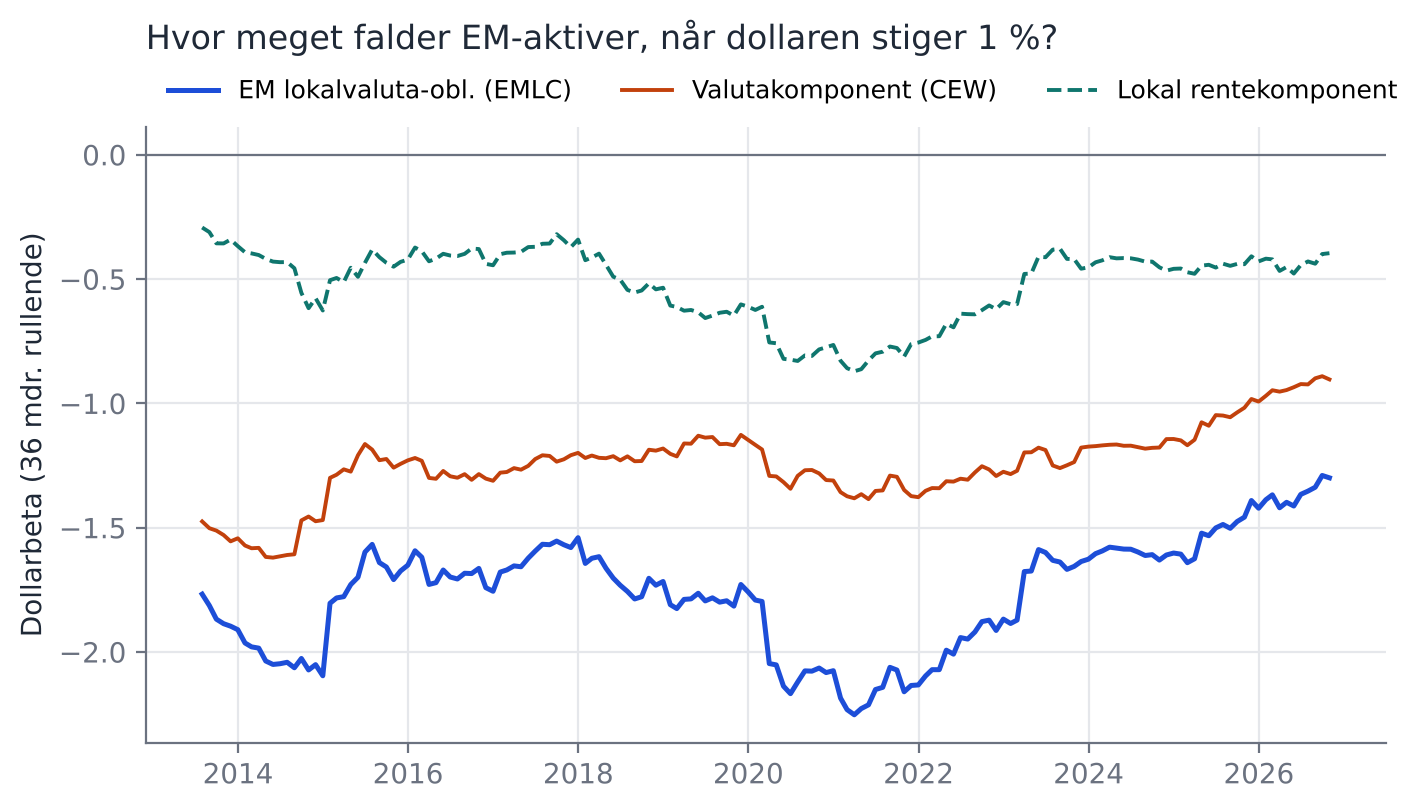
\includegraphics[width=0.9\textwidth]{fig_rullende_beta.png}
\caption{Rullende dollarbeta (36 måneder)}
\label{fig:roll}
\end{figure}

\subsection{Asymmetri}

Tabel~\ref{tab:asym} og figur~\ref{fig:asym} viser resultaterne fra ligning~\eqref{eq:asym}. For EMLC er betaen \AsymOp{} i måneder med stigende dollar og \AsymNed{} i måneder med faldende dollar. Forskellen går i den forventede retning, men testen af ens betaer giver $p=\AsymP$, så H4 \DomIV{} på 5\,\%-niveau. Testen har dog begrænset styrke. I simulationerne i bilag~\ref{app:mc} forkaster den kun i \MCPowEMLC\,\% af tilfældene, selv når der er en sand forskel på 0,4. Resultatet kan derfor ikke tolkes som evidens for, at effekten er symmetrisk.

Eksplorativt, og altså ikke fastlagt på forhånd, er forskellen signifikant for valutadelen. Spotkurven har en beta på \SpotOp{} med stigende dollar mod \SpotNed{} med faldende ($p=\NoVixPSpot$), og for CEW er $p=\NoVixPCEW$. En naturlig bekymring er, at måneder med stigende dollar ofte er krisemåneder, som marts 2020 og efteråret 2022, så asymmetrien kan handle om kriser snarere end om dollarens retning. Når der kontrolleres for ændringen i VIX, er $p$-værdien for spotkurven dog stadig \VixPSpot{} og for CEW \VixPCEW, jf.\ tabel~\ref{tab:robasym}. Asymmetrien i valutadelen kan altså ikke alene forklares af kriser målt ved VIX. Da resultatet er eksplorativt, bør det dog bekræftes på nye data, før der lægges vægt på det.

\begin{table}[h]
\centering
\small
\begin{threeparttable}
\caption{Asymmetri i dollarfølsomheden}
\label{tab:asym}
\begin{tabular}{lcccc}
\toprule
 & EMLC & CEW & Lokal rente & EMB \\
\midrule
$\beta^{op}$ & $-1{,}90^{***}$ & $-1{,}40^{***}$ & $-0{,}50^{***}$ & $-1{,}34^{***}$ \\
 & $(-11{,}48)$ & $(-14{,}92)$ & $(-4{,}00)$ & $(-4{,}63)$ \\
$\beta^{ned}$ & $-1{,}43^{***}$ & $-1{,}05^{***}$ & $-0{,}38^{***}$ & $-0{,}68^{***}$ \\
 & $(-9{,}31)$ & $(-10{,}45)$ & $(-3{,}51)$ & $(-2{,}72)$ \\
\midrule
$p$-værdi, $\beta^{op}=\beta^{ned}$ & \ensuremath{0{,}09} & \ensuremath{0{,}03} & \ensuremath{0{,}57} & \ensuremath{0{,}17} \\
Måneder med stigende dollar & 91 & 91 & 91 & 91 \\
Måneder med faldende dollar & 104 & 104 & 104 & 104 \\
\bottomrule
\end{tabular}

\begin{tablenotes}\footnotesize
\item \textit{Note:} Estimation af ligning~\eqref{eq:asym}. Newey-West $t$-værdier i parentes. $p$-værdien er fra en Wald-test af $\beta^{op}=\beta^{ned}$. Kun kolonnen EMLC er forhåndsfastlagt (H4).
\end{tablenotes}
\end{threeparttable}
\end{table}

\begin{figure}[h]
\centering
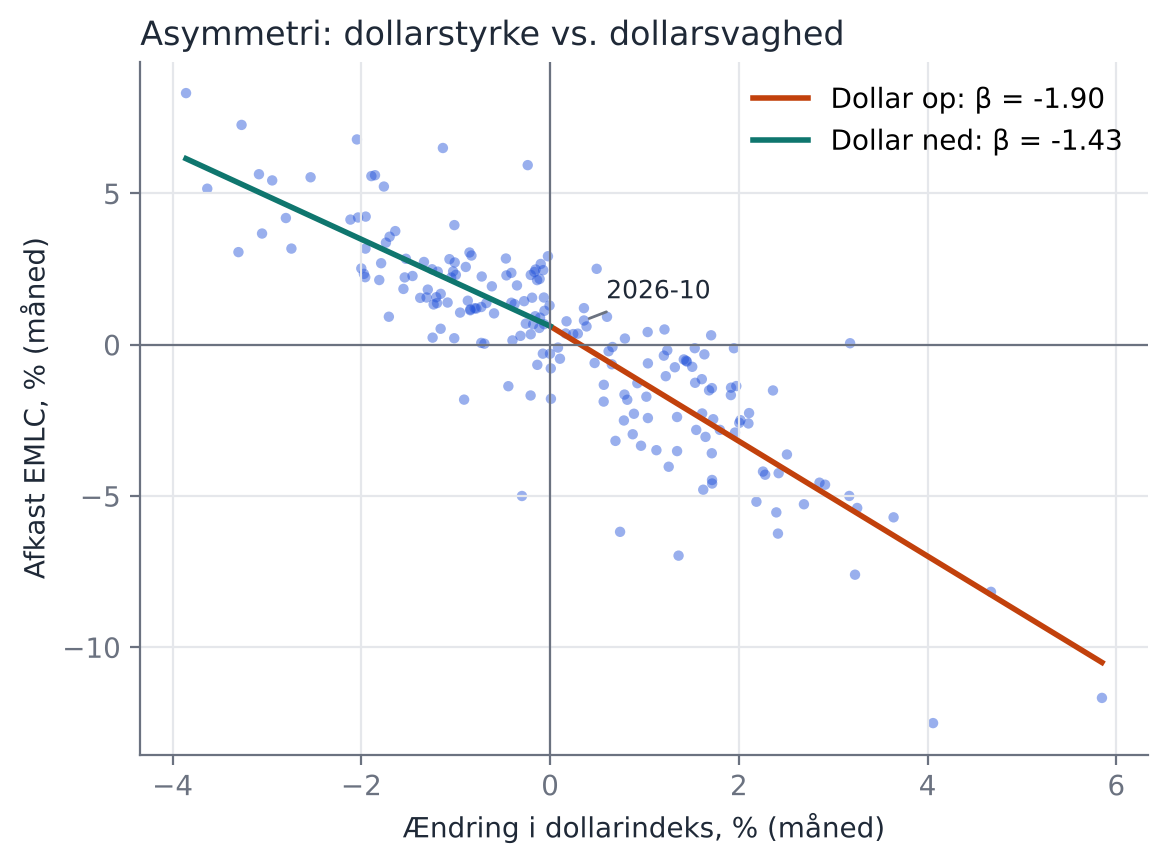
\includegraphics[width=0.72\textwidth]{fig_asymmetri.png}
\caption{EMLC-afkast mod ændringen i dollarindekset}
\label{fig:asym}
\end{figure}

\subsection{Kan dollaren forudsige afkastet?}

Tabel~\ref{tab:oos} viser, at sidste måneds dollarændring ikke giver en bedre forudsigelse end det historiske gennemsnit. For EMLC er $R^2_{OOS}=\OosRto\,\%$ med en Clark-West $p$-værdi på \OosP, så H5 \DomV. Den negative $R^2_{OOS}$ betyder, at modellen faktisk forudsiger dårligere end blot at bruge gennemsnittet. Der findes altså ingen evidens for, at dollareksponeringen kan udnyttes som et handelssignal med en måneds forsinkelse. Eksponeringen viser sig samtidig, og den er dermed en risiko, man bærer, snarere end en mulighed, man kan time.

\begin{table}[h]
\centering
\small
\begin{threeparttable}
\caption{Forudsigelse out-of-sample}
\label{tab:oos}
\begin{tabular}{lcccc}
\toprule
Aktiv & $R^2_{OOS}$ (\%) & Clark-West $t$ & $p$ (ensidet) & $N_{OOS}$ \\
\midrule
EMLC & \ensuremath{-1{,}51} & \ensuremath{-1{,}36} & \ensuremath{0{,}91} & 134 \\
CEW & \ensuremath{-2{,}79} & \ensuremath{-0{,}67} & \ensuremath{0{,}75} & 134 \\
Lokal rente & \ensuremath{-0{,}41} & \ensuremath{0{,}03} & \ensuremath{0{,}49} & 134 \\
EMB & \ensuremath{-0{,}97} & \ensuremath{-0{,}98} & \ensuremath{0{,}84} & 134 \\
\bottomrule
\end{tabular}

\begin{tablenotes}\footnotesize
\item \textit{Note:} $r_{i,t+1}$ regresseres på $\Delta\mathrm{USD}_t$ i et udvidende vindue (mindst 60 måneder). Benchmark er det historiske gennemsnit. Ensidet test af \citet{clark2007}.
\end{tablenotes}
\end{threeparttable}
\end{table}

\subsection{Dollarvendingen i efteråret 2026}

Følgende afsnit undersøger, om den seneste dollarvending opførte sig, som den historiske sammenhæng tilsiger. I \SepMonth{} steg dollarindekset \SepUSD\,\%, og EMLC gav et afkast på \SepEMLC\,\%. Tabel~\ref{tab:ep} sammenligner de faktiske afkast i de seneste tre måneder med modellen fra ligning~\eqref{eq:main}, estimeret \emph{uden} disse måneder, så sammenligningen er et ægte kontrafaktisk scenarie.

I september ventede modellen et afkast på \SepEMLCmodel\,\% for EMLC mod et faktisk afkast på \SepEMLC\,\%, mens EMB gav \SepEMB\,\% mod ventet \SepEMBmodel\,\%. \SepTekst{} Det er dog vigtigt at pointere, at en enkelt måned indeholder betydelig støj, og at forskellen derfor ikke kan tolkes som en systematisk ændring i sammenhængen.

\begin{table}[h]
\centering
\small
\begin{threeparttable}
\caption{Faktiske og modelforventede afkast i den seneste episode}
\label{tab:ep}
\begin{tabular}{llcccc}
\toprule
Måned & $\Delta\mathrm{USD}$ & Aktiv & Faktisk & Model & Afvigelse \\
\midrule
August 2026 & \ensuremath{-0{,}95} & EMLC & \ensuremath{1{,}06} & \ensuremath{1{,}73} & \ensuremath{-0{,}67} \\
 &  & CEW & \ensuremath{0{,}66} & \ensuremath{1{,}36} & \ensuremath{-0{,}71} \\
 &  & EMB & \ensuremath{0{,}55} & \ensuremath{0{,}80} & \ensuremath{-0{,}25} \\
\addlinespace
September 2026 & \ensuremath{2{,}01} & EMLC & \ensuremath{-2{,}58} & \ensuremath{-3{,}56} & \ensuremath{0{,}98} \\
 &  & CEW & \ensuremath{-1{,}22} & \ensuremath{-1{,}85} & \ensuremath{0{,}63} \\
 &  & EMB & \ensuremath{-3{,}80} & \ensuremath{-2{,}47} & \ensuremath{-1{,}33} \\
\addlinespace
Oktober 2026 & \ensuremath{0{,}36} & EMLC & \ensuremath{0{,}80} & \ensuremath{0{,}19} & \ensuremath{0{,}61} \\
 &  & CEW & \ensuremath{0{,}56} & \ensuremath{-0{,}31} & \ensuremath{0{,}87} \\
 &  & EMB & \ensuremath{1{,}24} & \ensuremath{1{,}41} & \ensuremath{-0{,}18} \\
\bottomrule
\end{tabular}

\begin{tablenotes}\footnotesize
\item \textit{Note:} Modellen inkluderer olie og US-renter og er estimeret på data før de viste måneder. Procent.
\end{tablenotes}
\end{threeparttable}
\end{table}

% ------------------------------------------------------------------ 4 Robusthed
\section{Robusthed}\label{sec:rob}

Følgende afsnit undersøger, om hovedresultaterne afhænger af valget af dollarindeks og valutaproxy. Analyserne var ikke fastlagt på forhånd.

\paragraph{Dollarindeks uden EM-valutaer.} Feds brede indeks har store vægte på blandt andet kinesisk yuan og mexicansk peso. En del af sammenhængen mellem indekset og EM-valutaerne er derfor mekanisk, fordi de samme valutaer indgår på begge sider af regressionen. Tabel~\ref{tab:robdollar} gentager estimationen med indekset mod avancerede økonomier, som ikke indeholder EM-valutaer. Dollarbetaen for EMLC falder fra \BetaEMLC{} til \AfeEMLC{} ($t=\TAfeEMLC$), og forklaringsgraden falder fra \RtoEMLC{} til \AfeRtoEMLC. For CEW falder $R^2$ fra \BredRtoCEW{} til \AfeRtoCEW. Det giver et indtryk af, hvor meget af den oprindelige forklaringsgrad der var mekanisk. Sammenhængen er dog stadig stærk og signifikant for alle aktiver, og restposten har en beta på \AfeLok{} ($t=\TAfeLok$). Hovedresultatet holder dermed.

\begin{table}[h]
\centering
\small
\begin{threeparttable}
\caption{Dollarbetaer med to dollarindeks}
\label{tab:robdollar}
\begin{tabular}{lcccccc}
\toprule
 & \multicolumn{3}{c}{Bredt indeks (inkl.\ EM)} & \multicolumn{3}{c}{Avancerede økonomier} \\ \cmidrule(lr){2-4}\cmidrule(lr){5-7}
Aktiv & $\beta$ & $t$ & $R^2$ & $\beta$ & $t$ & $R^2$ \\
\midrule
EMLC & $-1{,}70^{***}$ & $(-19{,}41)$ & \ensuremath{0{,}74} & $-1{,}27^{***}$ & $(-13{,}18)$ & \ensuremath{0{,}55} \\
CEW & $-1{,}25^{***}$ & $(-20{,}18)$ & \ensuremath{0{,}80} & $-0{,}95^{***}$ & $(-13{,}05)$ & \ensuremath{0{,}61} \\
Spotkurv (7 GBI-EM) & $-1{,}13^{***}$ & $(-21{,}13)$ & \ensuremath{0{,}79} & $-0{,}83^{***}$ & $(-13{,}14)$ & \ensuremath{0{,}56} \\
EMLC - CEW & $-0{,}45^{***}$ & $(-7{,}88)$ & \ensuremath{0{,}29} & $-0{,}32^{***}$ & $(-7{,}13)$ & \ensuremath{0{,}19} \\
EMLC - spotkurv & $-0{,}56^{***}$ & $(-11{,}82)$ & \ensuremath{0{,}36} & $-0{,}44^{***}$ & $(-9{,}93)$ & \ensuremath{0{,}29} \\
EMB & $-1{,}05^{***}$ & $(-7{,}28)$ & \ensuremath{0{,}42} & $-0{,}77^{***}$ & $(-6{,}98)$ & \ensuremath{0{,}30} \\
\bottomrule
\end{tabular}

\begin{tablenotes}\footnotesize
\item \textit{Note:} Bredt indeks: FRED \texttt{DTWEXBGS}. Avancerede økonomier: FRED \texttt{DTWEXAFEGS}. Newey-West $t$-værdier i parentes.
\end{tablenotes}
\end{threeparttable}
\end{table}

\paragraph{Valutaproxy.} Tabel~\ref{tab:robdek} sammenligner opdelingen med CEW og med spotkurven. Valutaandelen ligger mellem \AndelMin{} og \AndelMax\,\%, og restposten er negativ og signifikant i begge tilfælde.

\begin{table}[h]
\centering
\small
\begin{threeparttable}
\caption{Opdeling med to valutaproxyer}
\label{tab:robdek}
\begin{tabular}{lccccc}
\toprule
Valutaproxy & $\beta^{valuta}$ & $\beta^{rest}$ & $t^{rest}$ & Valutaandel & Korr.\ med EMLC \\
\midrule
CEW (ligevægtet, inkl. carry) & \ensuremath{-1{,}25} & \ensuremath{-0{,}45} & $(-7{,}88)$ & \ensuremath{74}\,\% & \ensuremath{0{,}93} \\
Spotkurv (7 GBI-EM, uden carry) & \ensuremath{-1{,}13} & \ensuremath{-0{,}56} & $(-11{,}82)$ & \ensuremath{67}\,\% & \ensuremath{0{,}92} \\
\bottomrule
\end{tabular}

\begin{tablenotes}\footnotesize
\item \textit{Note:} Valutaandel $=\beta^{valuta}/\beta^{EMLC}$. Restposten er EMLC minus valutaproxyen. Newey-West $t$-værdi i parentes.
\end{tablenotes}
\end{threeparttable}
\end{table}

\paragraph{Asymmetri og kriser.} Tabel~\ref{tab:robasym} viser asymmetritesten med og uden kontrol for ændringen i VIX.

\begin{table}[h]
\centering
\small
\begin{threeparttable}
\caption{Asymmetri med kontrol for VIX (eksplorativt)}
\label{tab:robasym}
\begin{tabular}{llcccc}
\toprule
Aktiv & VIX-kontrol & $\beta^{op}$ & $\beta^{ned}$ & Forskel & $p$ \\
\midrule
EMLC & nej & \ensuremath{-1{,}90} & \ensuremath{-1{,}43} & \ensuremath{-0{,}47} & \ensuremath{0{,}09} \\
 & ja & \ensuremath{-1{,}79} & \ensuremath{-1{,}37} & \ensuremath{-0{,}42} & \ensuremath{0{,}12} \\
CEW & nej & \ensuremath{-1{,}40} & \ensuremath{-1{,}05} & \ensuremath{-0{,}35} & \ensuremath{0{,}03} \\
 & ja & \ensuremath{-1{,}30} & \ensuremath{-1{,}00} & \ensuremath{-0{,}30} & \ensuremath{0{,}05} \\
Spotkurv (7 GBI-EM) & nej & \ensuremath{-1{,}29} & \ensuremath{-0{,}93} & \ensuremath{-0{,}36} & \ensuremath{0{,}01} \\
 & ja & \ensuremath{-1{,}25} & \ensuremath{-0{,}91} & \ensuremath{-0{,}34} & \ensuremath{0{,}02} \\
\bottomrule
\end{tabular}

\begin{tablenotes}\footnotesize
\item \textit{Note:} Ligning~\eqref{eq:asym} med og uden $\Delta\mathrm{VIX}_t$ som kontrol. $p$ fra Wald-test af $\beta^{op}=\beta^{ned}$. Ikke forhåndsfastlagt.
\end{tablenotes}
\end{threeparttable}
\end{table}

% ------------------------------------------------------------------ 5 Diskussion
\section{Diskussion}

Analysen påviser en stærk negativ sammenhæng mellem dollaren og afkastet på EM-obligationer i lokalvaluta. Det rejser spørgsmålet om, hvorvidt sammenhængen kan tolkes kausalt.

Regressionerne er samtidige, og dollaren er ikke tilfældigt tildelt. Både dollaren og EM-aktiverne påvirkes af global risikovillighed, amerikansk pengepolitik og vækstforventninger. Når investorerne bliver mere risikoaverse, søger de mod dollaren som sikker havn og sælger samtidig ud af EM. Det er derfor vanskeligt at opstille et klart kontrafaktisk scenarie, hvor dollaren ændrer sig, mens alt andet er uændret. Betaerne skal derfor tolkes som eksponering og ikke som kausale effekter. For en investor er det dog netop eksponeringen, der er relevant, fordi den beskriver, hvordan porteføljen opfører sig, når dollaren bevæger sig, uanset årsagen.

Den interne validitet af opdelingen i valuta- og rentedel trues af, at ingen af valutaproxyerne matcher EMLC's sammensætning. At restposten er negativ med to forskellige proxyer, styrker fortolkningen af en rentekanal, men det udelukker ikke, at en del skyldes vægtforskelle. En mere præcis opdeling kræver GBI-EM-indekset i en valutasikret og en ikke-valutasikret version.

Den eksterne validitet er ligeledes begrænset. Stikprøven dækker en periode med historisk lave renter og flere episoder med kraftige dollarbevægelser. Sammenhængen kan være anderledes i et regime med vedvarende højere amerikanske renter, som den renteforhøjelse, Federal Reserve gennemførte i september 2026, kan pege mod. Samtidig er resultaterne baseret på en bred kurv af EM-lande, og de kan ikke uden videre overføres til enkelte lande, hvis følsomhed afhænger af deres gæld i dollar, råvareeksport og pengepolitiske troværdighed.

Endelig bygger påstanden om forhåndsfastlagte hypoteser på tillid, da den ikke er dokumenteret med tidsstempler. Asymmetri-resultatet for valutadelen er desuden fundet efter, at den forhåndsfastlagte test for EMLC ikke var signifikant, og det er derfor mere usikkert, end $p$-værdierne alene antyder.

% ------------------------------------------------------------------ 6 Konklusion
\section{Konklusion}

Denne analyse har undersøgt, hvor følsomme EM-obligationer i lokalvaluta er over for den amerikanske dollar, og gennem hvilken kanal effekten virker. Resultaterne viser, at en stigning på 1\,\% i dollaren er forbundet med et afkast på \BetaEMLC\,\% med Feds brede indeks og \AfeEMLC\,\% med et indeks uden EM-valutaer. Lokalvaluta er markant mere dollarfølsom end hård valuta, hvilket er i overensstemmelse med teorien.

Valutaen står for mellem \AndelMin{} og \AndelMax\,\% af følsomheden, og restposten er negativ uanset valutaproxy. Det er konsistent med en rentekanal, men opdelingen er ikke præcis nok til at fastslå dens størrelse. \KonklAsym{} \KonklSignal{} Desuden smitter amerikanske renter tydeligt af på EM-obligationer, særligt i hård valuta.

Samlet set viser analysen, at en position i EM-obligationer i lokalvaluta i praksis også er en position på en svagere dollar. Analysens centrale bidrag er således at kvantificere denne eksponering, at vise at den holder på tværs af dollarindeks og valutaproxyer, og at tydeliggøre, hvor langt de offentligt tilgængelige data kan bære en opdeling i valuta- og rentekanal.

\bibliographystyle{plainnat}
\bibliography{references}

% ------------------------------------------------------------------ Bilag
\newpage
\appendix
\section{Validering af koden}\label{app:mc}

For at sikre, at koden regner rigtigt, er hele analysen kørt på \MCR{} syntetiske datasæt med kendte parametre. Monte Carlo-standardfejl står i parentes.

De gennemsnitlige estimater er $\hat\beta^{op}=\MCBetaOp$ og $\hat\beta^{ned}=\MCBetaNed$ mod sande værdier på $-1{,}0$ og $-0{,}6$, og $\hat\beta^{EMB}=\MCBetaEMB$ mod sand $-0{,}4$. Estimaterne er altså centreret om de sande værdier.

Under nulhypotesen om ingen forudsigelseskraft forkaster Clark-West-testen i \MCCWsize\,\% (\MCCWsizeSE) af tilfældene mod nominelt 5\,\%, så den er let konservativ. Asymmetritesten forkaster i \MCSizeAsym\,\% (\MCSizeAsymSE) af tilfældene, når den sande effekt er symmetrisk, hvilket er tæt på det nominelle niveau. Ved en sand forskel på 0,4 har testen en styrke på \MCPowEMLC\,\% (\MCPowEMLCSE) for EMLC og \MCPowCEW\,\% (\MCPowCEWSE) for CEW.

\section{Deklaration for anvendelse af generative AI-værktøjer}

\begin{tabular}{@{}ll@{}}
$\boxtimes$ & Jeg har benyttet generativ AI som hjælpemiddel/værktøj \\
$\square$ & Jeg har IKKE benyttet generativ AI som hjælpemiddel/værktøj \\
\end{tabular}

\medskip
\textbf{Benyttede værktøjer:} Claude (Anthropic), \url{https://claude.ai}

\textbf{Anvendelse:} Claude er anvendt til programmering af datahentning og estimation, til den statistiske validering og til udkast til tekst og opsætning i \LaTeX. Problemstillingen, valget af data, gennemgangen af resultaterne og fortolkningen er mine egne, og jeg har gennemgået og godkendt al kode og tekst.

\end{document}
